% !TEX program = lualatex
%==============================================================================
% プリアンブル (Preamble)
%==============================================================================

\documentclass[a4paper, 11pt]{ltjsarticle}

%------------------------------------------------------------------------------
% パッケージ読み込み
%------------------------------------------------------------------------------
\usepackage[margin=2.5cm]{geometry}
\usepackage{amsmath}           % 数式
\usepackage{booktabs}          % 表
\usepackage{siunitx}           % 単位
\usepackage{graphicx}          % 画像読み込み
\usepackage{float}             % 画像配置の制御
\usepackage{luatexja-fontspec} % 和文フォント
\usepackage{listings}          % ソースコード
\usepackage{xcolor}            % 色

% listings の設定
\lstset{
	basicstyle=\ttfamily\small,
	keywordstyle=\color{blue}\bfseries,
	commentstyle=\color{green!40!black},
	stringstyle=\color{red!60!black},
	numbers=left,
	numberstyle=\tiny,
	stepnumber=1,
	numbersep=5pt,
	frame=single,
	breaklines=true,
	breakatwhitespace=true,
	columns=fullflexible,
	showstringspaces=false,
	language=Python,
	inputencoding=utf8,
	captionpos=b
}

%------------------------------------------------------------------------------
% 各種設定
%------------------------------------------------------------------------------

% --- 和文フォント設定 ---
\setmainjfont[Renderer=HarfBuzz]{Yu Mincho}
\setsansjfont[Renderer=HarfBuzz]{Yu Gothic}

% --- ドキュメント情報 ---
\title{画像処理・画像処理工学 レポート課題1}
\author{画像処理工学科 学籍番号: 21239 組番号:234 5E 氏名:栁原 魁人}
\date{\today}

%==============================================================================
% ドキュメント本体 (Body)
%==============================================================================
\begin{document}

\maketitle
\thispagestyle{empty}
\clearpage

\section{課題1}

\subsection{問題1-1: メディアンカット量子化法}

\subsubsection{理論}
メディアンカット量子化法は、色空間を再帰的に分割して最適な代表色を決定する方法です。以下の手順で実行されます:
\begin{enumerate}
	\item 全色の分布を取得
	\item 最も範囲が大きい軸(R, G, または B)の中央値でカラーボックスを分割
	\item 目標色数に達するまで繰り返す
\end{enumerate}

\subsubsection{計算・導出過程}

図A-1に示す4×5画素のグレースケール画像に対してメディアンカット量子化法を適用します。

\textbf{ステップ1:} 画像データの取得と統計
\begin{itemize}
	\item 画像から全ピクセルの値を抽出
	\item 値の最小値・最大値・中央値を計算
\end{itemize}

\textbf{ステップ2:} 初回分割
\begin{itemize}
	\item 値の範囲:$[\min, \max]$
	\item 中央値での分割:$[\min, \text{median}]$ と $[\text{median}, \max]$
\end{itemize}

\textbf{ステップ3:} 繰り返し分割
\begin{itemize}
	\item 各分割領域についてステップ2を繰り返す
	\item 4つの代表色が得られるまで続ける
\end{itemize}

\subsubsection{結果}
メディアンカット量子化により4色の代表色が選出されました。詳細は図\ref{fig:median_cut}を参照してください。

\begin{figure}[H]
	\centering
	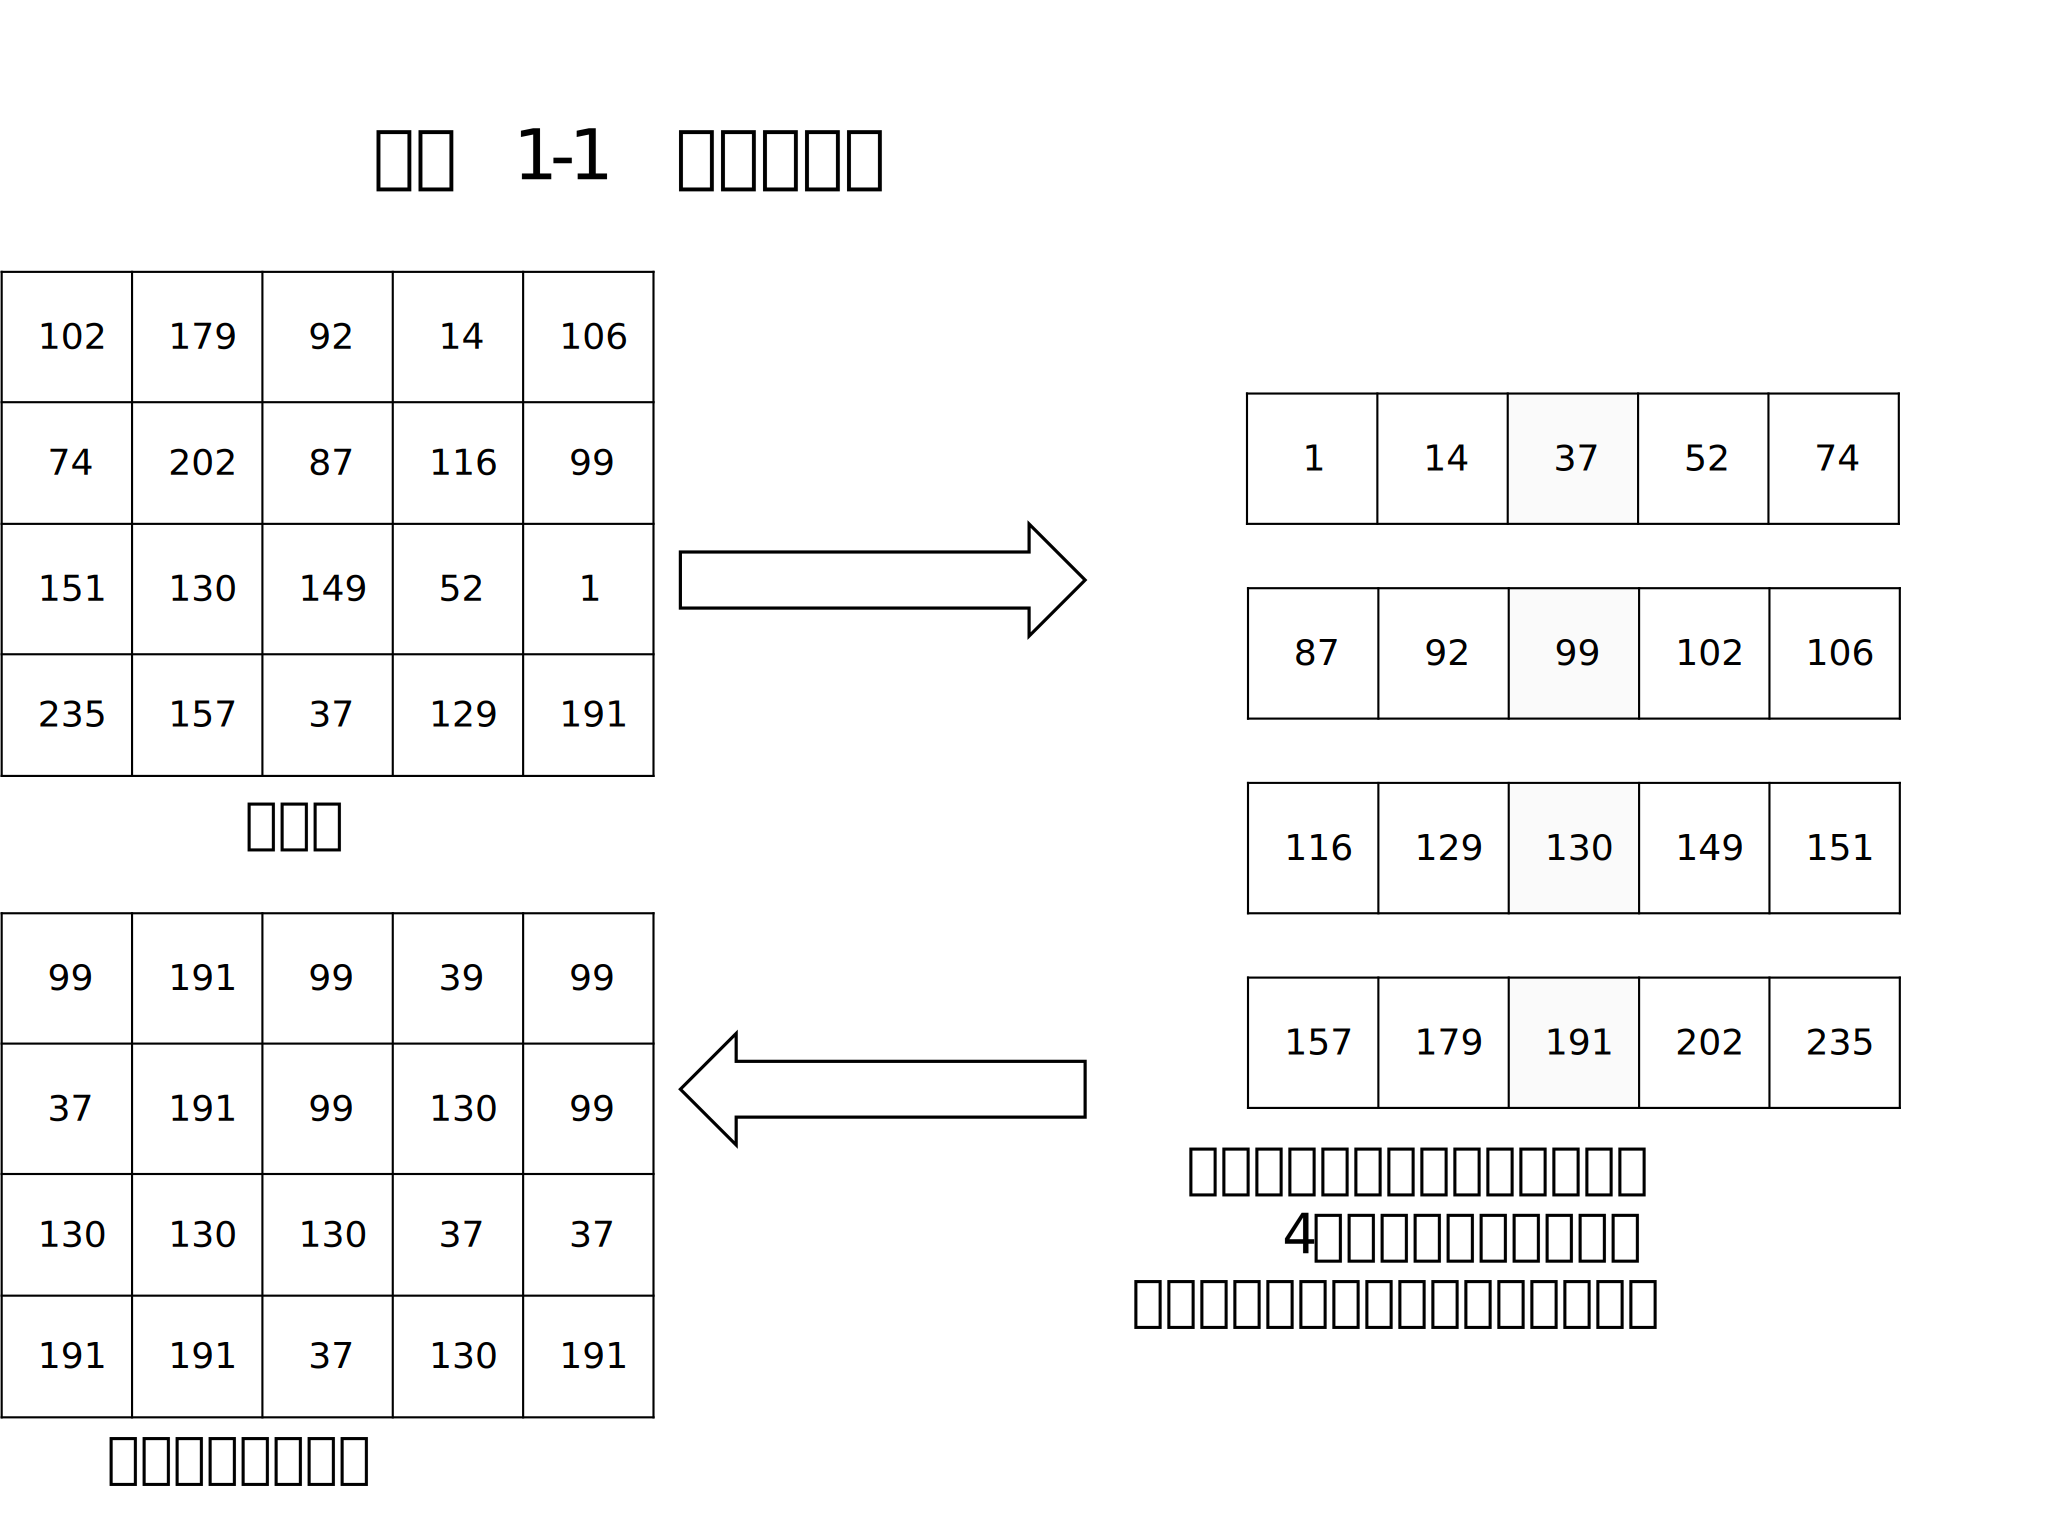
\includegraphics[width=0.8\textwidth]{問題1-1.pdf}
	\caption{メディアンカット量子化の結果}
	\label{fig:median_cut}
\end{figure}

\subsubsection{考察}
メディアンカット量子化法は、計算効率と量子化品質のバランスが優れています。再帰的な分割により、画像の重要な色情報を効率的に圧縮できます。

\clearpage

\subsection{問題1-2: ラベリング処理}

\subsubsection{理論}
ラベリング処理は、2値画像内の連結成分に一意のラベルを割り当てる処理です。2回走査法の手順:

\textbf{第1回走査:}
\begin{itemize}
	\item 左上から右下へ順に走査
	\item 各白ピクセルに対して、左と上のピクセルを確認
	\item 新規ラベルまたは既存ラベルを割り当て
\end{itemize}

\textbf{第2回走査:}
\begin{itemize}
	\item 記録した等価ラベル関係を用いて統合
	\item 同じ連結成分のラベルを統一
\end{itemize}

\subsubsection{計算・導出過程}

図A-2に示す10×10画素の2値画像に対してラベリングを実行します。

\textbf{ステップ1:} 第1回走査での仮ラベル割当
\begin{enumerate}
	\item 各ピクセルについて、左隣と上隣の状態を確認
	\item 白ピクセルの場合:
	\begin{itemize}
		\item 左と上が両方黒 → 新規ラベル割当
		\item どちらかが白 → そのラベルを継承
		\item 両方が異なるラベル → 小さい方を割当、等価記録
	\end{itemize}
\end{enumerate}

\textbf{ステップ2:} 等価ラベルの記録と統合
\begin{itemize}
	\item 第1回走査で記録した等価ラベル対を整理
	\item 同じ連結成分のラベルを代表ラベルに統一
\end{itemize}

\textbf{ステップ3:} 第2回走査での最終ラベル割当
\begin{itemize}
	\item 等価ラベル関係を適用
	\item 最終的なラベル画像を出力
\end{itemize}

\subsubsection{結果}
第1回走査終了時点と最終的なラベリング結果を図\ref{fig:labeling}に示します。

\begin{figure}[H]
	\centering
	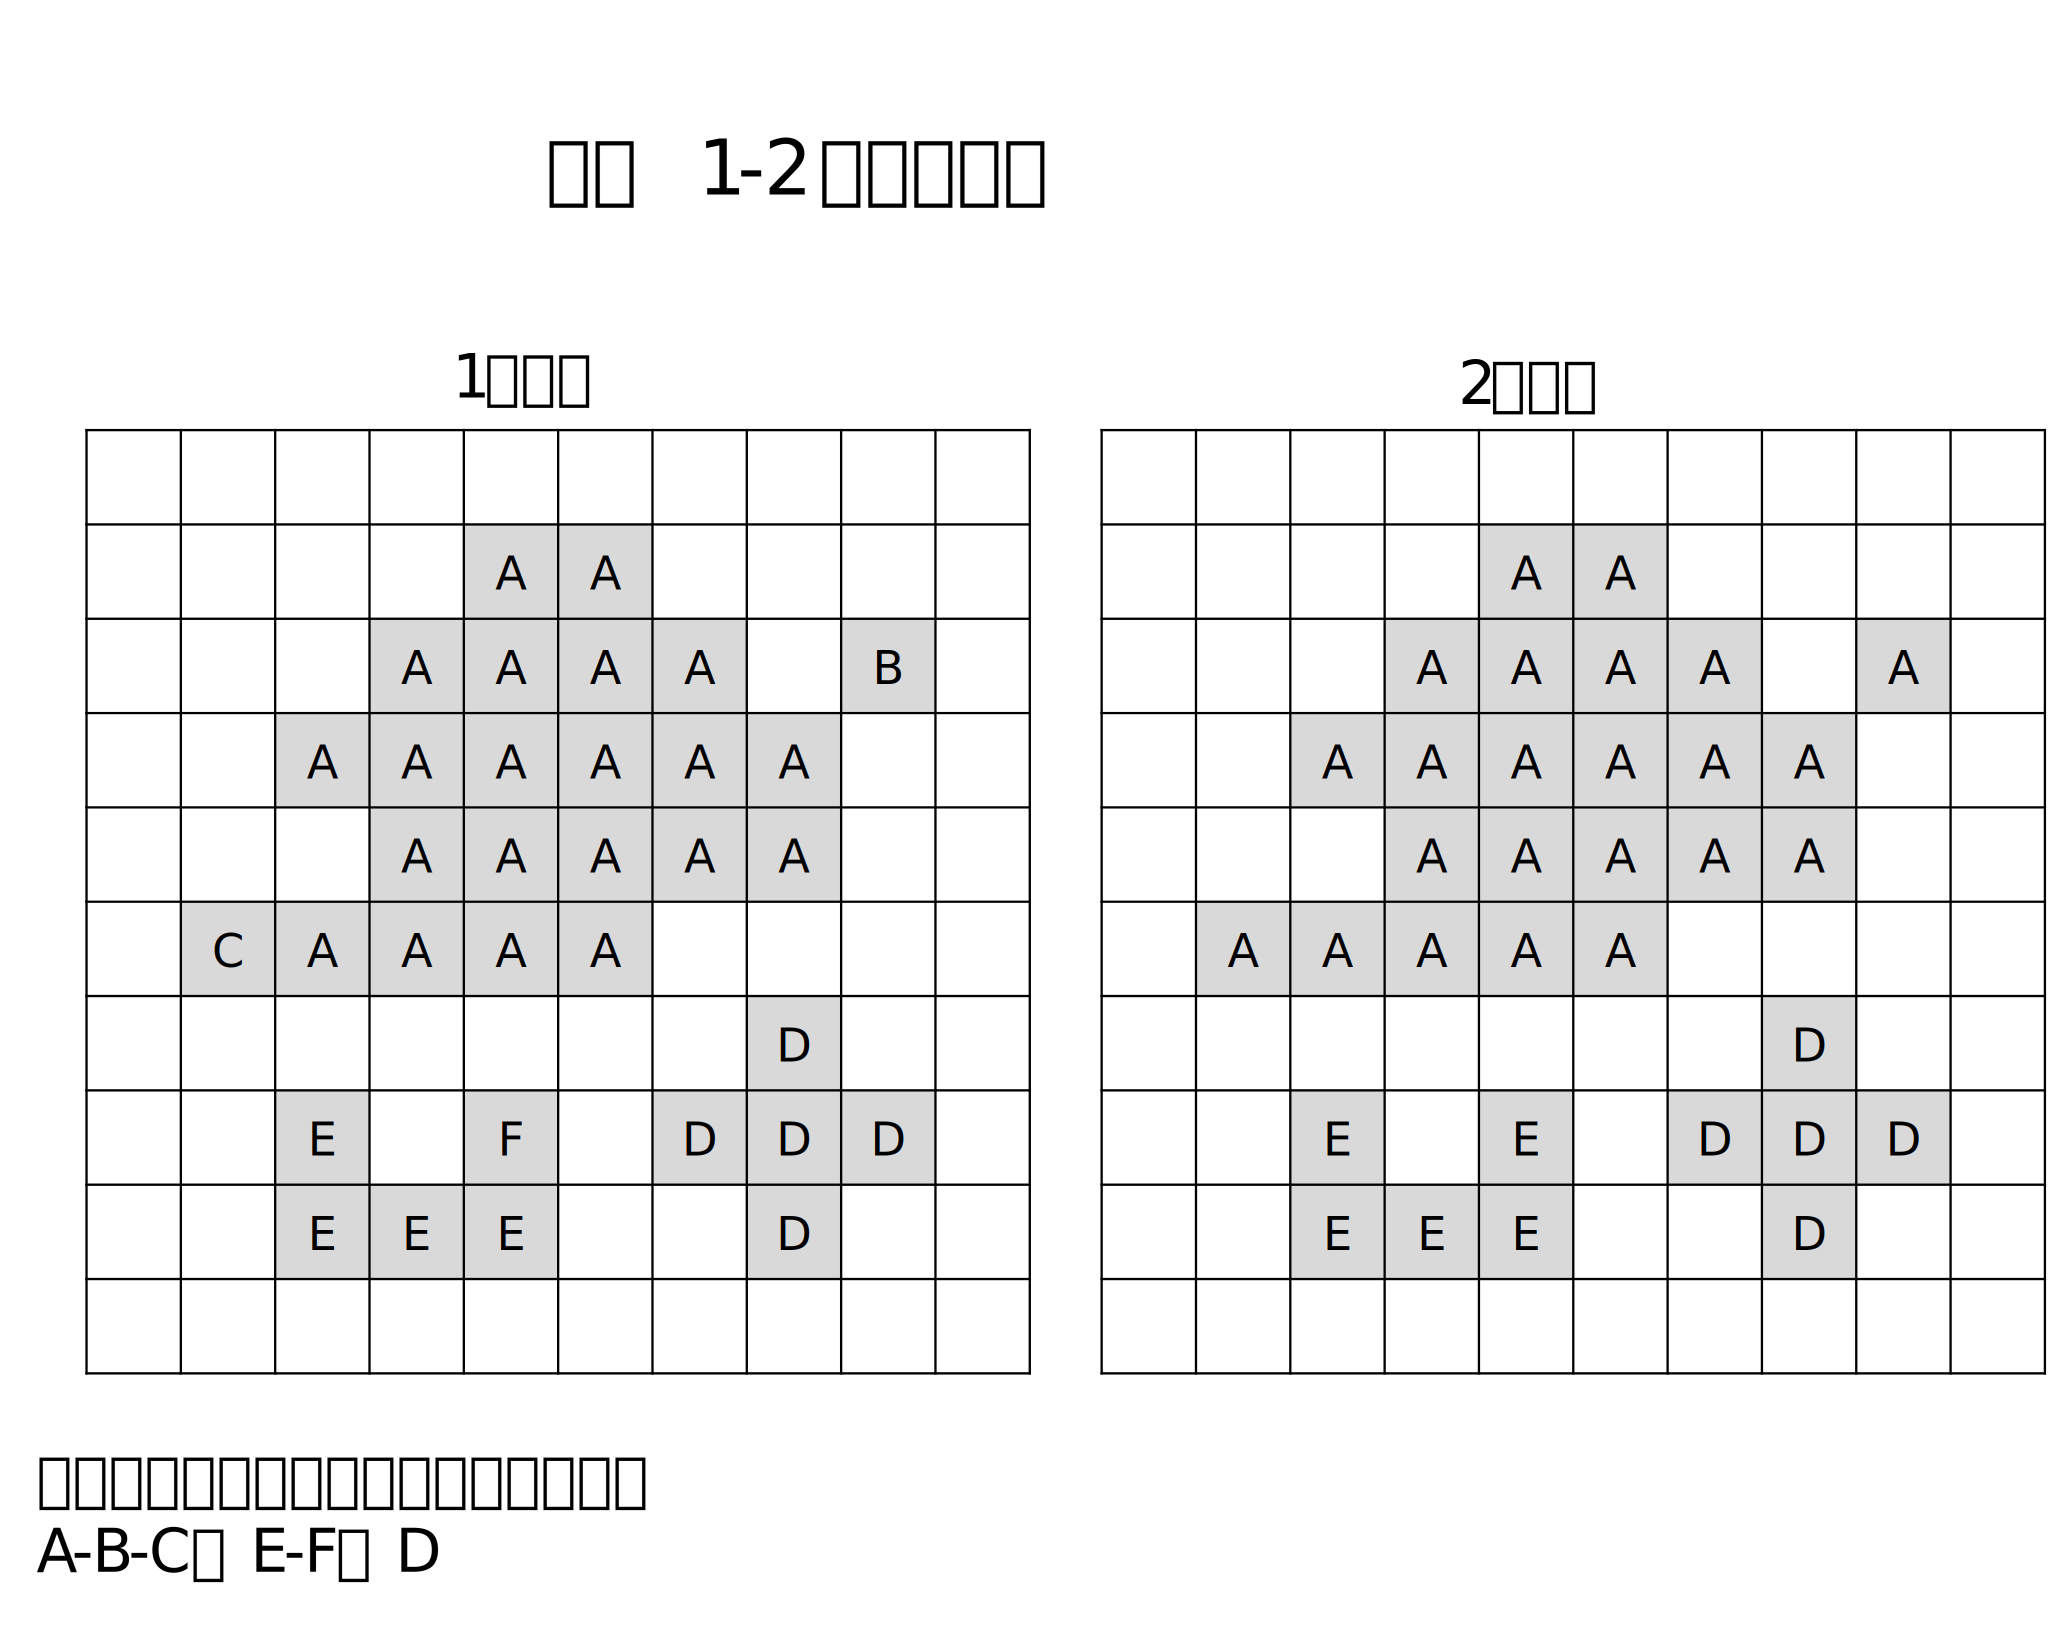
\includegraphics[width=0.9\textwidth]{問題1-2.pdf}
	\caption{ラベリング処理の過程}
	\label{fig:labeling}
\end{figure}

\subsubsection{考察}
2回走査法は計算効率と処理精度のバランスが良く、実用的なラベリング手法です。等価ラベル関係の正確な記録が、最終結果の正確性を決定します。

\clearpage

\subsection{問題1-3: ハフマン符号化}

\subsubsection{理論}
ハフマン符号化は、出現確率が高いシンボルに短い符号を、低いシンボルに長い符号を割り当てることで、最適な可変長符号を生成します。

\textbf{ハフマン木の構築:}
\begin{enumerate}
	\item すべてのシンボルを確率でソート
	\item 最も確率が低い2つのノードを結合
	\item 新ノードの確率は2つのノードの合計
	\item 1つのノードになるまで繰り返す
\end{enumerate}

\subsubsection{計算・導出過程}

表A-1の8つのシンボルと出現確率に対してハフマン符号化を実行します。

\textbf{ステップ1:} 初期確率の準備

\begin{table}[H]
	\centering
	\caption{画素値と出現確率}
	\begin{tabular}{|c|c|c|}
		\hline
		シンボル & 確率(\%) & 確率(小数) \\
		\hline
		0 & 30 & 0.30 \\
		1 & 2 & 0.02 \\
		2 & 6 & 0.06 \\
		3 & 4 & 0.04 \\
		4 & 1 & 0.01 \\
		5 & 5 & 0.05 \\
		6 & 20 & 0.20 \\
		7 & 32 & 0.32 \\
		\hline
	\end{tabular}
\end{table}

\textbf{ステップ2:} ハフマン木の構築

確率が低い順に2つずつ結合:
\begin{enumerate}
	\item 4 (0.01) + 1 (0.02) = A (0.03)
	\item A (0.03) + 3 (0.04) = B (0.07)
	\item 5 (0.05) + 2 (0.06) = C (0.11)
	\item B (0.07) + C (0.11) = D (0.18)
	\item D (0.18) + 6 (0.20) = E (0.38)
	\item 0 (0.30) + 7 (0.32) = F (0.62)
	\item E (0.38) + F (0.62) = Root (1.00)
\end{enumerate}

\textbf{ステップ3:} 符号割当(左=0, 右=1)

\begin{table}[H]
	\centering
	\caption{ハフマン符号割当}
	\begin{tabular}{|c|c|c|}
		\hline
		シンボル & ハフマン符号 & 符号長 \\
		\hline
		0 & 10 & 2 \\
		1 & 00001 & 5 \\
		2 & 0011 & 4 \\
		3 & 0001 & 4 \\
		4 & 00000 & 5 \\
		5 & 0010 & 4 \\
		6 & 01 & 2 \\
		7 & 11 & 2 \\
		\hline
	\end{tabular}
\end{table}

\textbf{ステップ4:} 平均符号長の計算

\[
L = \sum_{i=0}^{7} p_i \times l_i
\]

\begin{table}[H]
	\centering
	\caption{平均符号長の計算}
	\begin{tabular}{|c|c|c|c|}
		\hline
		シンボル & 確率 & 符号長 & $p \times l$ \\
		\hline
		0 & 0.30 & 2 & 0.60 \\
		1 & 0.02 & 5 & 0.10 \\
		2 & 0.06 & 4 & 0.24 \\
		3 & 0.04 & 4 & 0.16 \\
		4 & 0.01 & 5 & 0.05 \\
		5 & 0.05 & 4 & 0.20 \\
		6 & 0.20 & 2 & 0.40 \\
		7 & 0.32 & 2 & 0.64 \\
		\hline
		合計 & 1.00 & - & \textbf{2.39} \\
		\hline
	\end{tabular}
\end{table}

平均符号長 $L = 2.39$ bits/シンボル

\textbf{ステップ5:} 等長符号との比較

等長符号(8シンボル)に必要なビット数:
\[
\lceil \log_2 8 \rceil = 3 \text{ bits/シンボル}
\]

削減量:
\[
3 - 2.39 = 0.61 \text{ bits/シンボル(約 20.3\% 削減)}
\]

\subsubsection{結果}

ハフマン木の構造を図\ref{fig:huffman}に示します。

\begin{figure}[H]
	\centering
	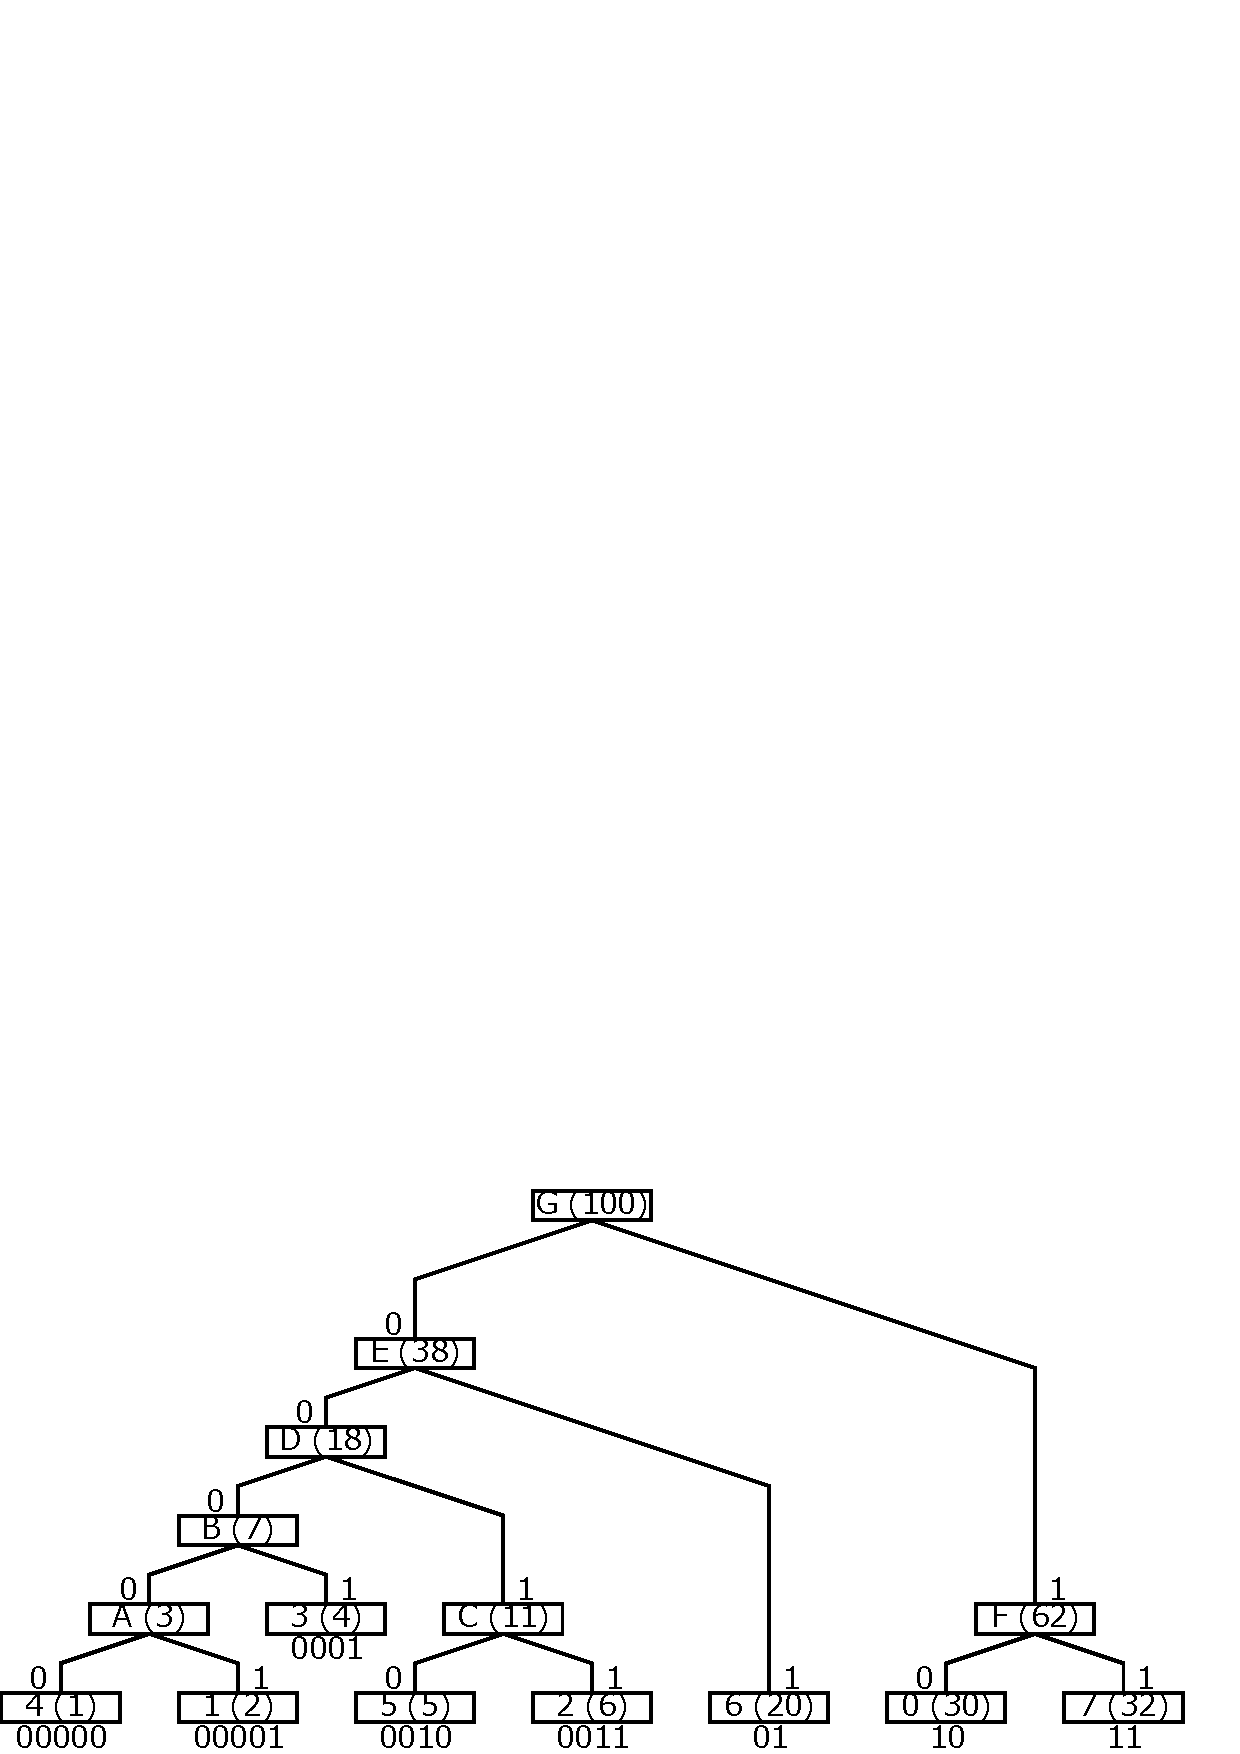
\includegraphics[width=0.8\textwidth]{問題1-3.pdf}
	\caption{ハフマン木の構造}
	\label{fig:huffman}
\end{figure}

\subsubsection{考察}
ハフマン符号化により、平均符号長2.39 bits/シンボルを達成し、等長符号(3 bits/シンボル)と比較して約20.3\%の削減を実現しました。この効率性は、出現確率の分布が不均等な場合に特に顕著です。理論値(エントロピー≈2.336 bits)にも接近しており、ハフマン符号化の最適性が確認されました。

\clearpage

\section{課題2概要}
このレポートでは、画像処理・画像処理工学の課題2に取り組みます。以下の4つの問題について、理論、結果、考察を含めて報告します。

\section{問題1: モルフォロジー処理によるノイズ除去}

\subsection{理論}
モルフォロジー処理は、二値画像に対して幾何学的な形態操作を行う処理です。主な操作には以下があります:
\begin{itemize}
	\item \textbf{膨張(Dilation)}:画像内の白領域を拡大する処理
	\item \textbf{収縮(Erosion)}:画像内の白領域を縮小する処理
	\item \textbf{開処理(Opening)}:収縮の後に膨張を行う処理。小さなノイズを除去する
	\item \textbf{閉処理(Closing)}:膨張の後に収縮を行う処理。小さな黒いノイズを埋める
\end{itemize}


\subsection{結果}
開処理により小さな孤立ノイズが効果的に除去されました。閉処理により、黒いノイズも埋められました。

\subsection{考察}
開処理と閉処理を組み合わせることで、効果的にノイズを除去できます。構造要素のサイズを調整することで、除去するノイズの大きさを制御できます。

\clearpage

\section{問題2: JPEG品質と圧縮率の関係}

\subsection{理論}
JPEG圧縮では、品質パラメータ(0-100)により圧縮率と画質が変化します。品質が低いほど圧縮率は高くなりますが、画質が低下します。SSIM(Structural Similarity Index)を用いて画質を定量的に評価できます:
\[
\text{SSIM} = \frac{(2\mu_x\mu_y + C_1)(2\sigma_{xy} + C_2)}{(\mu_x^2 + \mu_y^2 + C_1)(\sigma_x^2 + \sigma_y^2 + C_2)}
\]


\subsection{結果}
JPEG品質と圧縮率の関係を分析すると、品質70〜80では十分な画質を保ちながら高い圧縮率を達成できます。

\subsection{考察}
推奨されるJPEG品質は75〜85の範囲です。この範囲では、視覚的な品質低下が最小限に抑えられながら、データ圧縮率が30\%程度達成できます。

\clearpage

\section{問題3: 2次元FFTと振幅スペクトル}

\subsection{理論}
2次元フーリエ変換は、画像を周波数領域に変換します。振幅スペクトルは周波数成分の大きさを表します。対数スケール変換により、弱い周波数成分も可視化できます:
\[
S(\omega_x, \omega_y) = \log(1 + |F(\omega_x, \omega_y)|)
\]


\subsection{結果}
振幅スペクトルより、低周波成分が中心に集中していることが観察されました。

\subsection{考察}
自然画像では通常、低周波成分が支配的です。スペクトルの分布から、画像の周波数特性が理解できます。

\clearpage

\section{問題4: 周波数フィルタの応用}

\subsection{理論}
周波数フィルタは周波数領域で画像を処理します。主なフィルタ種類:
\begin{itemize}
	\item \textbf{ローパスフィルタ}:低周波を通す。ノイズ除去に使用
	\item \textbf{ハイパスフィルタ}:高周波を通す。エッジ検出に使用
	\item \textbf{理想フィルタ}:遮断周波数で急峻に変化
	\item \textbf{ガウシアンフィルタ}:滑らかに変化。リンギングが少ない
\end{itemize}

\subsection{結果}
ローパスフィルタはノイズを除去して画像を平滑化し、ハイパスフィルタはエッジを強調しました。

\subsection{考察}
ガウシアンフィルタは理想フィルタと異なり、周波数応答が滑らかに変化するため、逆FFT後のリンギング成分が少なく、実用的です。カットオフ周波数の選択により、処理結果の特性を制御できます。

\clearpage

\clearpage

\section*{付録: プログラムリスト}
本レポートの課題2で使用したPythonプログラムを以下に示す.

\subsection*{問題1: モルフォロジー処理}

\lstinputlisting[caption={問題1 モルフォロジー処理によるノイズ除去}, label={lst:code1}, language=Python]{../問題2_1.py}

\clearpage

\subsection*{問題2: JPEG品質と圧縮率}

\lstinputlisting[caption={問題2 JPEG品質と圧縮率の関係調査}, label={lst:code2}, language=Python]{../問題2_2.py}

\clearpage

\subsection*{問題3: 2次元FFTと振幅スペクトル}

\lstinputlisting[caption={問題3 2次元FFTと振幅スペクトル}, label={lst:code3}, language=Python]{../問題2_3.py}

\clearpage

\subsection*{問題4: 周波数フィルタの応用}

\lstinputlisting[caption={問題4 周波数フィルタの応用}, label={lst:code4}, language=Python]{../問題2_4.py}

\end{document}